% Standalone compilation wrapper for gw_section_body.tex
% Mirrors the host paper's class and macros so the drop-in renders as it
% would inside Latex_writting/Hydrodynamical combustion/Main.tex.
% Compile: latexmk -pdf gw_section_standalone.tex
\documentclass[10pt,superscriptaddress,amsmath,aps,prc,twocolumn,nofootinbib,floatfix]{revtex4-1}

\usepackage{amssymb}
\usepackage{amsmath}
\usepackage{graphicx}
\usepackage{xcolor}

% Macros copied from the host paper's preamble
\newcommand{\m}{\text{m}}
\newcommand{\km}{\text{km}}
\newcommand{\s}{\text{s}}
\newcommand{\MeV}{\text{MeV}}
\newcommand{\kHz}{\text{kHz}}
\newcommand{\nsat}{\ensuremath{n_{0}}}

% Editorial-comment macros copied from the host paper's preamble
\newcommand{\AHcom}[1]{\textsf{\color{cyan}{\textsuperscript{AH}#1}}}
\newcommand{\JS}[1]{{\color{violet}#1}}
\newcommand{\JScom}[1]{\textsf{\color{violet} [\textsuperscript{JS}#1]}}

% Fake labels for cross-references into the host paper (resolved for real
% once the body is \input into Main.tex; here they render as II, III, IV).
\makeatletter
\newcommand{\hostlabel}[2]{\protected@write\@auxout{}{\string\newlabel{#1}{{#2}{1}}}}
\makeatother

\begin{document}

\section{Postmerger gravitational wave peak frequency shift}
\label{sec:gw}

The postmerger gravitational-wave spectrum of a neutron-star merger usually has a single peak at $f_{\rm peak}\approx2$--$4\,\kHz$, which comes from the fundamental quadrupolar ($m=2$) oscillation of the remnant \cite{Stergioulas:2011gd,Takami:2014tva}.
Simulations find that compared with purely hardronic matter, having an instantaneous first-order transition to quark matter would shifts $f_{\rm peak}$ by several hundred Hz \cite{Bauswein:2018bma,Most:2018eaw,Weih:2019xvw,Bauswein:2020ggy,Fujimoto:2022xhv,Espino:2023llj}.
All of these simulations convert nuclear matter the instant its pressure exceeds $p_\text{crit}$, which is the instantaneous-conversion described in the introduction.
Here we estimate how the finite phase boundary speed obtained in Sec.~\ref{sec:results} changes that prediction.
We write $f_{\rm peak}^{\infty}$ for the peak frequency under instantaneous conversion and $f_{\rm peak}^{\rm finite}$ for the peak frequency when the nuclear to quark phase transition is limited by boundary propagation speed we calculated.

\textbf{Quark matter fraction under a finite-speed conversion.}
At each time $t$, we define region where quark matter is thermodynamically favored by
\begin{equation}
\Omega_{\rm crit}(t)
=\left\{\boldsymbol{x}:\,P(\boldsymbol{x},t)>p_\text{crit}\right\},
\label{eq:critical_region}
\end{equation}
with $p_\text{crit}$ determined as in Sec.~\ref{sec:results}.
The instantaneous prescription converts all of $\Omega_{\rm crit}$ at every instant.
With a finite conversion speed, metastable nuclear matter in $\Omega_{\rm crit}$ converts only after the phase boundary has swept over it, which we track with an indicator field $I_q(\boldsymbol{x},t)$: $I_q=1$ where there's deconfined quark matter and $I_q=0$ elsewhere.
Matter with $P>p_\text{crit}$ and $I_q=0$ is the metastable nuclear matter whose conversion speed we calculated in Sec.~\ref{sec:speed}.
We assume that converted matter stays converted if the local pressure later falls back below $p_\text{crit}$.

%The motion of the boundary in the merger frame follows from Sec.~\ref{sec:speed}.
%The front advances into the nuclear matter at speed $u(0^-)$ relative to nuclear matter, so the boundary moves with the local fluid velocity plus $u(0^-)$ along the boundary's normal direction, towards the nuclear phase.
%For merger relavant temperature $\leq 50$ MeV and metastability, the calculated speeds obey $u(0^-)\lesssim10^{-5}$ in natural units, so we do not distinguish between proper and ordinary 3-velocity in this section.
%Advection by the merger flow rearranges the boundary but does not convert nuclear matter; the converted volume grows only through the normal propagation at $u(0^-)$.
%In a simulation, $I_q$ can be implemented as a marker (level-set) field transported with this velocity; Appendix~\ref{sec:finite_rate_implementation} gives the prescription.

We measure the progress of conversion by the converted volume fraction of the critical-pressure region,
\begin{equation}
X_q(t)
=\frac{1}{V_{\rm crit}(t)}
\int_{\Omega_{\rm crit}(t)}I_q(\boldsymbol{x},t)\,dV\,,
\label{eq:converted_fraction}
\end{equation}
where $V_{\rm crit}(t)$ is the volume of $\Omega_{\rm crit}(t)$.
The same definition can be weighted by baryon density, or by the local sensitivity of the $m=2$ mode to the equation of state \AHcom{what does this mean?}\JScom{The index $m$ is the azimuthal mode number.
A perturbation of a nearly axisymmetric remnant can be expanded in the angle $\phi$ about the rotation axis into terms that vary as $e^{i(m\phi-\omega t)}$, and $m$ counts how many full cycles the pattern completes in one turn around that axis.
An $m=0$ pattern is axisymmetric, a breathing or quasi-radial motion; $m=1$ is a one-sided displacement; $m=2$ stretches the equatorial cross-section into a rotating bar.
Only the bar radiates appreciably.
Gravitational-wave emission has no monopole or dipole part, so it comes from the mass quadrupole, and within the quadrupole the $m=2$ component has a time-varying moment while the $m=0$ (axisymmetric) component does not.
Strictly, $m$ fixes only the azimuthal shape: the dominant peak is the $\ell=m=2$ fundamental mode, with smaller $m=2$ contributions from higher multipoles $\ell=3,4,\dots$
A pattern $\propto e^{i(2\phi-\omega t)}$ rotates rigidly at angular speed $\omega/2$ and looks the same after half a turn, so a distant observer sees the quadrupole repeat twice per revolution and the wave emerges at $f_{\rm peak}=\omega/2\pi$.}, without changing the estimates below.

Evaluating $X_q$ requires a geometry for $\Omega_{\rm crit}$, sketched in Fig.~\ref{fig:omega_crit_geom}.
We assume that each of the two inspiraling neutron stars already has a quark-matter core of radius $R_0$.
When the stars merge, the remnant keeps a double-core structure for the first few milliseconds, so in the equatorial plane $\Omega_{\rm crit}$ splits into two congruent lobes that wrap around one another, making a taiji (yin--yang) shape with one of the original stellar cores, at the center of each lobe.
This is the same $m=2$ deformation that carries the mass quadrupole responsible for the postmerger GW emission, so the converted fraction and its mode-weighted variant refer to the same region.
The pattern corotates with the fluid, so rotation carries the lobes around without converting any matter.
The two quark cores that the stars bring in are the seeds, and we are not considering strange quark matter nucleation here.
Each core boundary then advances into the surrounding metastable nuclear matter at speed $u(0^-)$, so over the postmerger emission window $\Delta t_{\rm pm}$ the core radius grows from $R_0$ to $R_0+u(0^-)\,\Delta t_{\rm pm}$, and
\begin{equation}
X_q
=
\left[\frac{R_0+u(0^-)\,\Delta t_{\rm pm}}{R_{\rm lobe}}\right]^{3}
\,,\quad X_q \leq 1
\label{eq:lobe_fraction}
\end{equation}
where $R_{\rm lobe}\equiv[3V_{\rm crit}/(8\pi)]^{1/3}$ is the effective radius of one lobe and $V_{\rm crit}$ the total volume of $\Omega_{\rm crit}$.
The pre-merger cores set the baseline $X_q(u{=}0)=(R_0/R_{\rm lobe})^3$.
The part the front adds is a thin shell: for $u(0^-)\,\Delta t_{\rm pm}\ll R_0$ each core gains a volume $4\pi R_0^{2}\,u(0^-)\,\Delta t_{\rm pm}$, linear in the front speed rather than cubic.

\begin{figure}[t]
  \centering
  \IfFileExists{Plots/omega_crit_taiji_3d.pdf}{%
    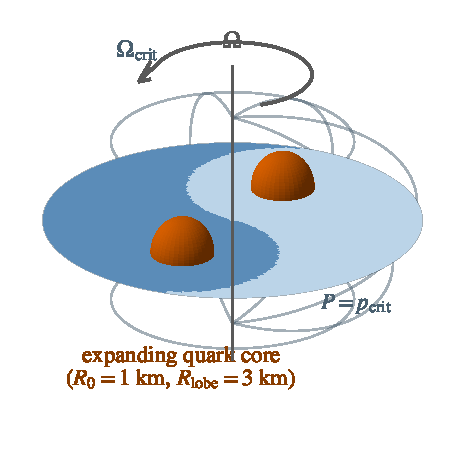
\includegraphics[width=1\columnwidth]{Plots/omega_crit_taiji_3d.pdf}%
  }{%
    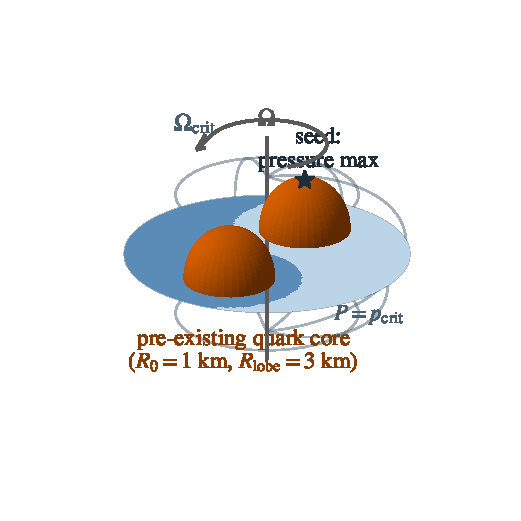
\includegraphics[width=1\columnwidth]{omega_crit_taiji_3d.pdf}%
  }
  \caption{Geometry of the critical-pressure region $\Omega_{\rm crit}$ in the early remnant.
  The cage of rings is the $P=p_{\rm crit}$ surface of the oblate remnant core.
  The equatorial cut shows the two congruent lobes of the rotating $m=2$ double-core pattern (taiji shape); the two tones only distinguish the lobes, which hold the same metastable nuclear matter.
  Each lobe carries one of the pre-merger quark cores (shaded spheres, drawn to scale for $R_0=1\,\km$ and $R_{\rm lobe}=3\,\km$).
  Over the emission window the conversion front advances each core boundary by only $u(0^-)\,\Delta t_{\rm pm}\approx10\,\m$.}
  \label{fig:omega_crit_geom}
\end{figure}

\textbf{Catch-up within the emission window.}
$f_{\rm peak}^{\rm finite}$ meets $f_{\rm peak}^{\infty}$ only if the front reaches every point of $\Omega_{\rm crit}$ within that window. 
And to achieve this, the front velocity $u(0^-)$ should satisfy:
\begin{equation}
u(0^-)\gtrsim\frac{L_{\rm max}}{\Delta t_{\rm pm}}
\quad\Longrightarrow\quad
f_{\rm peak}^{\rm finite}\simeq f_{\rm peak}^{\infty}\,,
\label{eq:catch_up}
\end{equation}
where $L_{\rm max}$ is longest diatance the phase boundary has to swipe over to convert the entire $\Omega_{\rm crit}$ to quark matter. %largest propagation distance, measured through the matter, from the initial seed surface to any point of $\Omega_{\rm crit}$.

Both sides of Eq.~\eqref{eq:catch_up} are fixed by known numbers.
Quark cores in instantaneous-conversion simulations extend over a few kilometers \cite{Most:2018eaw,Bauswein:2018bma}; as reference values we take the radius of merger medium with pressure greater than $p_{\rm crit}$ to be $R_{\rm lobe}=3\,\km$ and each merging neutron star has a quark core of radius $R_0=1\,\km$, and the postmerger peak is accumulated over $\Delta t_{\rm pm}\approx5$--$20\,\text{ms}$ of emission \cite{Takami:2014tva,Vretinaris:2019spn}.
The the core boundary is the phase boundary, and the farthest matter sits at the tip of the wrapping tail, so $L_{\rm max}\approx2R_{\rm lobe}-R_0\approx5\,\km$ and catching up requires $u(0^-)\gtrsim3\times10^{5}$--$10^{6}\,\m\,\s^{-1}$.
The maximum boundary speeds of Sec.~\ref{sec:results} at merger temperatures, $u_{\rm max}(0^-)\approx10^{2}$--$10^{3}\,\m\,\s^{-1}$, fall short by factors of $300$ to $10^{4}$.
This is the quantitative form of the concern raised in the introduction: the instantaneous prescription implicitly assumes boundary speeds near $10^{6}\,\m\,\s^{-1}$, while weak-interaction-limited propagation reaches at most $10^{3}\,\m\,\s^{-1}$.
The front therefore barely moves the converted fraction.
For $u(0^-)\sim 10^{3}\,\m\,\s^{-1}$ and $\Delta t_{\rm pm}\sim 10\,\text{ms}$ each core radius grows by $\sim 10\,\m$, which is about one percent of $R_0$, and Eq.~\eqref{eq:lobe_fraction} moves $X_q$ only from the baseline $(R_0/R_{\rm lobe})^3=0.037$ to $0.038$.

On the timescale of the postmerger emission, weak-interaction-limited conversion is frozen: the phase boundary is a comoving surface, and outside the two quark matter cores $\Omega_{\rm crit}$ stays metastable nuclear matter.
Interface-mode analyses of the inspiral assume the same frozen composition \cite{Tonetto:2020bie,Counsell:2025hcv,Pereira:2025xsi}; here it follows from the microphysics under merger conditions.
Converting the whole core within the window would instead need seeds spread through the volume, spaced by no more than $\sim2\,u_{\rm max}(0^-)\,\Delta t_{\rm pm}\approx20\,\m$.
Whether nucleation can supply that seed density is a question of bubble-nucleation physics rather than boundary propagation, and we do not address it here.
Hydrodynamic instabilities of the front could also raise the effective conversion rate above our planar bound, as discussed in Sec.~\ref{sec:conclusion}.

\textbf{Peak-frequency shift and observability.}
Let $\Delta f_{\rm PT}$ denote the signed shift of the peak frequency between a remnant whose critical-pressure region $\Omega_{\rm crit}$ is fully converted and one that is purely metastable nuclear matter, so $\Delta f_{\rm PT}\equiv f_{\rm peak}^{\infty}-f_{\rm peak}(X_q{=}0)$.
The state $X_q=0$ is a reference point rather than a realized configuration, because both stars arrive with quark cores.
Under the instantaneous-conversion assumption of the existing simulations $\Delta f_{\rm PT}$ is an equilibrium quantity fixed by the equation of state: a pure nuclear matter EoS run gives $f_{\rm peak}(X_q{=}0)$, and a hybrid EoS run that switches to quark matter above $p_{\rm crit}$ gives $f_{\rm peak}^{\infty}$.
Such simulations find $|\Delta f_{\rm PT}|$ of several hundred Hz for strong first-order transitions \cite{Bauswein:2018bma,Most:2018eaw,Weih:2019xvw,Prakash:2023afe}.
$\Delta f_{\rm PT}$ can also be read off observationally, as a deviation of $f_{\rm peak}$ from hadronic empirical relations of the form $f_{\rm peak}^{\infty}=F(\mathcal{M}_{\rm chirp},R_{1.8})$, where $\mathcal{M}_{\rm chirp}$ is the chirp mass and $R_{1.8}$ the radius of a cold, nonrotating $1.8\,M_\odot$ star \cite{Bauswein:2012ya,Vretinaris:2019spn}.

To place the finite-rate peak frequency $f_{\rm peak}^{\rm finite}$ between $f^\infty_{\rm peak}$ and $f_{\rm peak}(X_q{=}0)$, we argue that the peak frequency shifts $\Delta f_{\rm peak}$ and the reference $\Delta f_{\rm PT}$ are related by the converted fraction $X_q$.
Converting a volume element replaces nuclear matter by quark matter, which changes the local pressure-density relation and therefore the restoring force and inertia of the mode.
For a small converted volume these shifts add over the converted region, so if the mode has roughly uniform sensitivity across $\Omega_{\rm crit}$ the frequency moves in proportion to $X_q$,
\begin{equation}
\begin{aligned}
f_{\rm peak}^{\rm finite}
&\simeq
f_{\rm peak}(X_q{=}0)+X_q(\Delta t_{\rm pm})\,\Delta f_{\rm PT}
\\
&=
f_{\rm peak}^{\infty}-\bigl[1-X_q(\Delta t_{\rm pm})\bigr]\,\Delta f_{\rm PT}\,,
\end{aligned}
\label{eq:finite_peak_frequency}
\end{equation}
where $X_q$ is the total quark-matter fraction inside $\Omega_{\rm crit}$, including the pre-merger quark cores.
To better understand this, if $X_q = 0$, which means there's no quark matter, and the two stars don't even have quark cores to begin with. 
In this case, $\Delta f_{\rm peak} = \Delta f_{\rm PT}$, but we know from Eq.~\eqref{eq:lobe_fraction} that $X_q\geq (R_0/R_{\rm lobe})^3$ since we assume that the two stars have quark cores.
On the other hand, if $X_q = 1$, which means all matter in $\Omega_{\rm crit}$ is converted to quark matter, then $f_{\rm peak}^{\rm finite} = f_{\rm peak}^{\infty}\ $, and $\Delta f_{\rm peak} = 0\ $.

The linear law is a leading-order approximation; terms nonlinear in $X_q$ describe higher-order changes in the mode structure and need simulations at intermediate converted fractions.
%Because the cores sit at the lobe centers, where the $m=2$ bar has its largest amplitude, their weight in the mode may exceed their volume fraction, so $X_q(u{=}0)\,\Delta f_{\rm PT}$ is a lower estimate of their contribution.
Subtracting Eq.~\eqref{eq:finite_peak_frequency} from $f_{\rm peak}^{\infty}$ gives the deficit,
\begin{equation}
\Delta f_{\rm peak}
\equiv
f_{\rm peak}^{\infty}-f_{\rm peak}^{\rm finite}
\simeq
\bigl[1-X_q\bigr]\,\Delta f_{\rm PT}\,.
\label{eq:rate_shift}
\end{equation}
Two effects set this deficit, and only one of them is the front speed.
The pre-merger cores already fill a fraction $X_q(\Delta t_{\rm pm}{=}0)=(R_0/R_{\rm lobe})^3=0.037$ of $\Omega_{\rm crit}$, which by itself leaves a deficit $[1-X_q(u{=}0)]\,\Delta f_{\rm PT}\approx0.96\,\Delta f_{\rm PT}$.
Over the emission window the finite front adds only $\Delta X_q\approx10^{-3}$ to $X_q$, a further shift of $\Delta X_q\,\Delta f_{\rm PT}\approx0.1$--$0.9\,$Hz.
The slow front is therefore dynamically frozen, and the large deficit reflects the small size of the pre-merger cores rather than the front speed.

Figure~\ref{fig:rate_deficit} shows $\Delta f_{\rm peak}$ as a function of the boundary speed, for six values of $\Delta f_{\rm PT}$ calibrated as endpoint differences from published instantaneous-conversion simulations \cite{Prakash:2023afe,Bauswein:2018bma}.
Across the calculated $u_{\rm max}(0^-)\approx10^{2}$--$10^{3}\,\m\,\s^{-1}$ the deficit stays near $0.96\,\Delta f_{\rm PT}$, so the shift predicted by instantaneous-conversion simulations is not realized and the instantaneous prescription misplaces the peak by nearly the full $|\Delta f_{\rm PT}|$.

\begin{figure}[t]
  \centering
  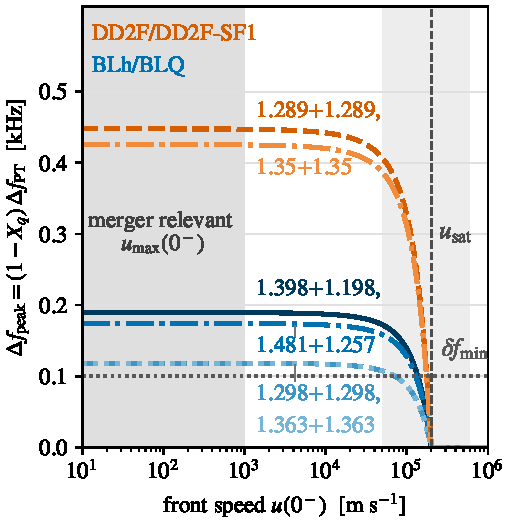
\includegraphics[width=\columnwidth]{Plots/f_peak.pdf}%
  \caption{Finite-rate frequency deficit $\Delta f_{\rm peak}=(1-X_q)\,\Delta f_{\rm PT}$ from Eqs.~\eqref{eq:lobe_fraction} and \eqref{eq:rate_shift}, using the pre-existing-core geometry with $R_0=1\,\km$, $R_{\rm lobe}=3\,\km$, and $\Delta t_{\rm pm}=10\,\text{ms}$.
  Each curve uses a $\Delta f_{\rm PT}$ calibrated as the endpoint difference between hybrid-EOS and purely hadronic instantaneous-conversion simulations, labeled by EOS pair and binary masses; five cases (all BLh/BLQ pairs and the DD2F/DD2F-SF1 $1.289{+}1.289$ pair) are from Table IV of \cite{Prakash:2023afe}, and the DD2F/DD2F-SF1 $1.35{+}1.35$ pair is from \cite{Bauswein:2018bma}.
  The two BLh/BLQ binaries with $\Delta f_{\rm PT}=0.123\,\kHz$ overlap.
  Neither reference reports the size of the quark-matter region, so we apply the same fiducial geometry to all six cases.
  The converted fraction $X_q(u(0^-))$ is then common to every curve and $\Delta f_{\rm PT}$ only rescales it, which is why the curves fall off together: the location of the fall-off is set by the geometry alone, not by the equation of state.
  The grey band on the left marks the maximum boundary speeds calculated in Sec.~\ref{sec:results} at merger temperatures.
  The dashed line is the saturation speed $u_{\rm sat}=(R_{\rm lobe}-R_0)/\Delta t_{\rm pm}$, above which the front would fill the lobes within the emission window, and the light band around it shows how far $u_{\rm sat}$ moves for $R_{\rm lobe}=2$--$4\,\km$ and $\Delta t_{\rm pm}=5$--$20\,\text{ms}$.
  Throughout the shaded band the deficit is $(1-X_q)\,\Delta f_{\rm PT}\approx0.96\,\Delta f_{\rm PT}=0.12$--$0.45\,\kHz$, above the $\delta f_{\rm min}\approx0.1\,\kHz$ resolution of a loud (postmerger signal-to-noise ratio ${\gtrsim}10$) next-generation detection \cite{Breschi:2022ens,Clark:2015zxa}.}
  \label{fig:rate_deficit}
\end{figure}

Whether this is detectable depends on the frequency resolution of postmerger observations.
The discrepancy is measurable if
\begin{equation}
\bigl[1-X_q\bigr]\,\bigl|\Delta f_{\rm PT}\bigr|
\gtrsim\delta f_{\rm min}\,,
\label{eq:observability}
\end{equation}
where $\delta f_{\rm min}$ is the smallest resolvable shift of the peak.
This resolution depends steeply on how loud the postmerger signal is.
For the Einstein Telescope, Bayesian recoveries of the peak frequency carry errors of order $1\,\kHz$ at postmerger signal-to-noise ratio $7$, roughly the detection threshold, but tighten to below $0.1\,\kHz$ at signal-to-noise ratio $10$ \cite{Breschi:2022ens}.
A Fisher estimate for a nearby source at ${\sim}30\,$Mpc with advanced LIGO gives a similar scale, $\delta f_{\rm peak}\approx50\,$Hz \cite{Clark:2015zxa}.
Bayesian model selection can distinguish phase-transition-induced shifts of this size \cite{Prakash:2023afe}.
We therefore take $\delta f_{\rm min}\approx0.1\,\kHz$ as the resolution of a loud postmerger detection.
The calibrated $|\Delta f_{\rm PT}|$ span $0.12$--$0.47\,\kHz$ and $1-X_q\approx0.96$, so the deficits are $0.12$--$0.45\,\kHz$ (Fig.~\ref{fig:rate_deficit}).
Equation~\eqref{eq:observability} then holds for every case once the postmerger signal-to-noise ratio reaches ${\sim}10$, while near the detection threshold the ${\sim}1\,\kHz$ errors would hide all of them.
A detected postmerger peak from a remnant that crosses the transition should therefore sit at the metastable hadronic value rather than at the shifted equilibrium value, unless nucleation seeds conversion densely enough to bypass the front-speed bound.

The inputs to this estimate (the geometry of $\Omega_{\rm crit}$, the emission window $\Delta t_{\rm pm}$, and the calibration $\Delta f_{\rm PT}$) all depend on the binary chirp mass, so Eqs.~\eqref{eq:finite_peak_frequency} and \eqref{eq:observability} define $f_{\rm peak}^{\rm finite}(\mathcal{M}_{\rm chirp},u(0^-))$ once those inputs come from equilibrium sequences or from numerical relativity.
We do not predict the strain amplitude of the peak; that requires the excitation energy and damping of the $m=2$ mode in addition to its frequency.

\appendix

\section{Implementing finite-rate conversion in merger simulations}
\label{sec:finite_rate_implementation}

The finite-rate prescription of Sec.~\ref{sec:gw} can be added to a hydrodynamic merger simulation with one additional advected field.
Let $\Phi(\boldsymbol{x},t)$ be a marker field whose zero surface is the phase boundary, with $\Phi>0$ in quark matter and $\Phi<0$ in nuclear matter, so that the conversion indicator is $I_q=\Theta(\Phi)$.
Only the zero surface and the sign of $\Phi$ are physical; its magnitude may be chosen for numerical convenience, e.g.\ by reinitializing $\Phi$ to the signed distance from the boundary.

The boundary moves with the local fluid velocity $\boldsymbol{v}$ plus the conversion speed $u(0^-)$ along the normal $\widehat{\boldsymbol{n}}=-\boldsymbol{\nabla}\Phi/|\boldsymbol{\nabla}\Phi|$, which points from the quark phase into the nuclear phase.
Requiring the zero surface to follow this velocity gives
\begin{equation}
\partial_t\Phi
+\boldsymbol{v}\boldsymbol{\cdot}\boldsymbol{\nabla}\Phi
=u(0^-)\,\bigl|\boldsymbol{\nabla}\Phi\bigr|\,,
\label{eq:marker_transport}
\end{equation}
a level-set equation whose source term converts matter at the calculated speed.
Here $\boldsymbol{v}$ is the fluid velocity on the nuclear side, because $u(0^-)$ is defined relative to the nuclear matter flowing into the front; the boundary speed relative to the quark side differs by the density ratio through baryon-flux conservation (Sec.~\ref{sec:speed}).
The speed $u(0^-)$ is evaluated pointwise on the boundary from the local values of $n_B(0^-)-n_B^{\rm crit}(T)$ and $T$, using the analytic boundary-speed formula of Sec.~\ref{sec:speed} or a tabulation of the numerical solutions.

Two limitations of the prescription mirror the physics.
First, $I_q=\Theta(\Phi)$ builds in hysteresis: where the front has passed, a later pressure drop below $p_\text{crit}$ does not undo the conversion unless a reverse-conversion speed is supplied on the quark side of the boundary.
Second, Eq.~\eqref{eq:marker_transport} transports existing boundaries only; where $P>p_\text{crit}$ but no boundary is present, conversion requires nucleation, which must be seeded explicitly.

\bibliographystyle{JHEP}
\bibliography{gw_refs}

\end{document}
